\documentclass{standalone}
\usepackage{tikz}
\usetikzlibrary{patterns, positioning}
\usepackage[sfdefault]{ClearSans} %% option 'sfdefault' activates Clear Sans as the default text font
\usepackage[T1]{fontenc}

\begin{document}
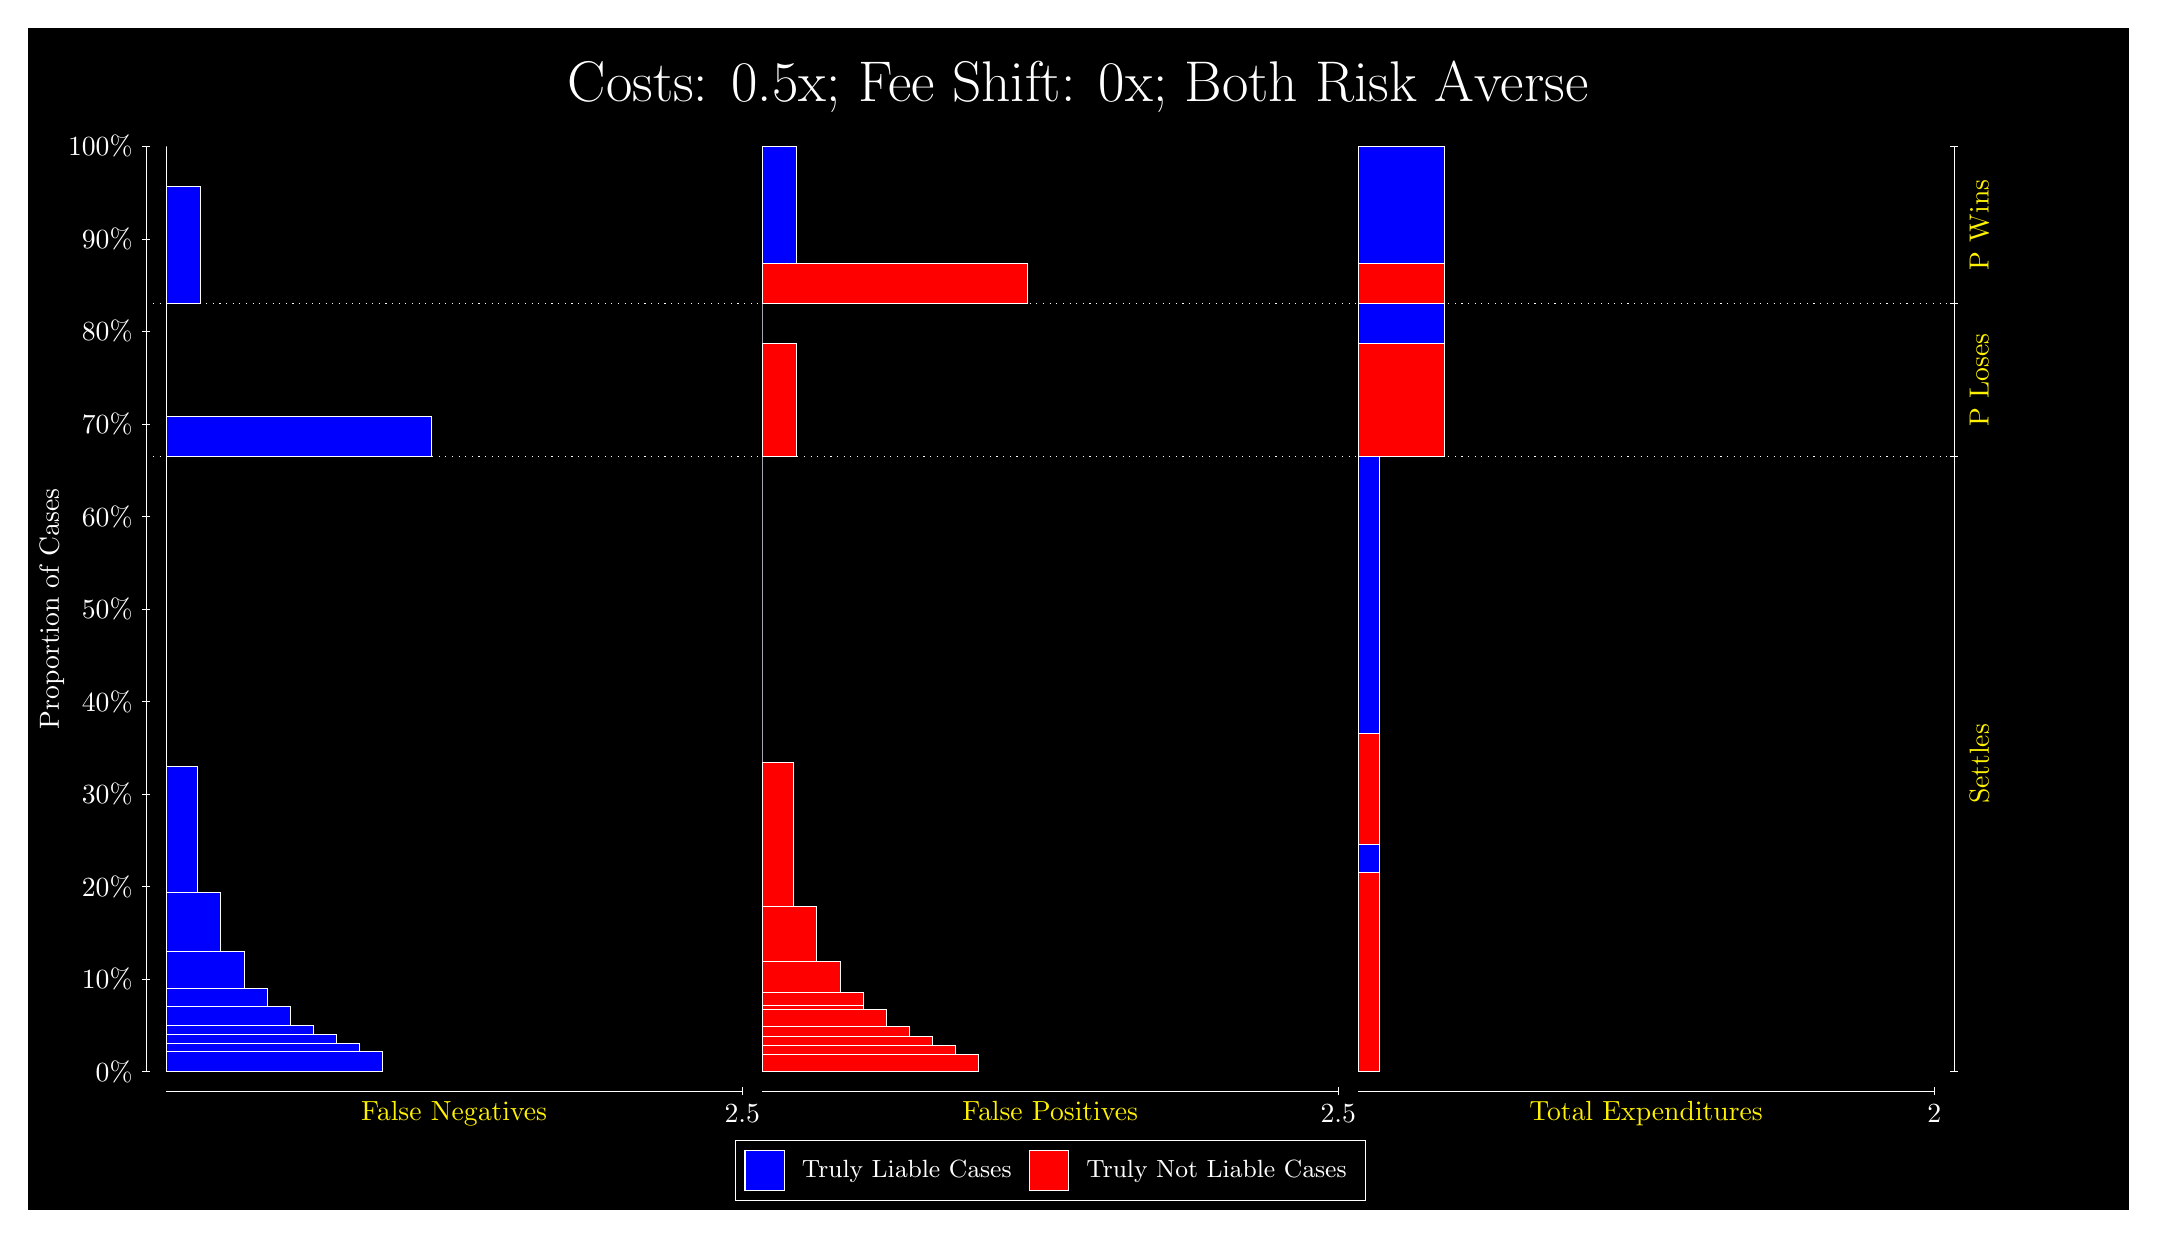
\begin{tikzpicture}
\draw[fill=black] (0,0) rectangle (26.667,15);
\draw[text=white] (0,13.5) rectangle (26.667,15) node[midway] {\huge Costs: 0.5x; Fee Shift: 0x; Both Risk Averse};
\draw[white, very thin] (1.5,1.75) -- (1.5,13.5);
\node[rotate=90, text=white, anchor=center] at (0.3, 7.625) {Proportion of Cases};
\draw[white, very thin] (1.45,1.75) -- (1.55,1.75);
\node[text=white, anchor=east] at (1.45, 1.75) {0\%};
\draw[white, very thin] (1.45,2.925) -- (1.55,2.925);
\node[text=white, anchor=east] at (1.45, 2.925) {10\%};
\draw[white, very thin] (1.45,4.1) -- (1.55,4.1);
\node[text=white, anchor=east] at (1.45, 4.1) {20\%};
\draw[white, very thin] (1.45,5.275) -- (1.55,5.275);
\node[text=white, anchor=east] at (1.45, 5.275) {30\%};
\draw[white, very thin] (1.45,6.45) -- (1.55,6.45);
\node[text=white, anchor=east] at (1.45, 6.45) {40\%};
\draw[white, very thin] (1.45,7.625) -- (1.55,7.625);
\node[text=white, anchor=east] at (1.45, 7.625) {50\%};
\draw[white, very thin] (1.45,8.8) -- (1.55,8.8);
\node[text=white, anchor=east] at (1.45, 8.8) {60\%};
\draw[white, very thin] (1.45,9.975) -- (1.55,9.975);
\node[text=white, anchor=east] at (1.45, 9.975) {70\%};
\draw[white, very thin] (1.45,11.15) -- (1.55,11.15);
\node[text=white, anchor=east] at (1.45, 11.15) {80\%};
\draw[white, very thin] (1.45,12.325) -- (1.55,12.325);
\node[text=white, anchor=east] at (1.45, 12.325) {90\%};
\draw[white, very thin] (1.45,13.5) -- (1.55,13.5);
\node[text=white, anchor=east] at (1.45, 13.5) {100\%};

\draw[white, very thin] (24.457,1.75) -- (24.457,13.5);
\draw[white, very thin] (24.407,1.75) -- (24.507,1.75);
\node[anchor=west] at (24.407, 1.75) {};
\draw[white, very thin] (24.407,9.5635) -- (24.507,9.5635);
\node[anchor=west] at (24.407, 9.5635) {};
\draw[white, very thin] (24.407,11.506) -- (24.507,11.506);
\node[anchor=west] at (24.407, 11.506) {};
\draw[white, very thin] (24.407,13.5) -- (24.507,13.5);
\node[anchor=west] at (24.407, 13.5) {};

\draw[white, very thin, fill=blue] (1.75,1.75) rectangle (4.4946,2.0025);
\draw[white, very thin, fill=blue] (1.75,2.0025) rectangle (4.2018,2.1137);
\draw[white, very thin, fill=blue] (1.75,2.1137) rectangle (3.9091,2.223);
\draw[white, very thin, fill=blue] (1.75,2.223) rectangle (3.6163,2.3419);
\draw[white, very thin, fill=blue] (1.75,2.3419) rectangle (3.3236,2.5767);
\draw[white, very thin, fill=blue] (1.75,2.5767) rectangle (3.0308,2.8024);
\draw[white, very thin, fill=blue] (1.75,2.8024) rectangle (2.738,3.2823);
\draw[white, very thin, fill=blue] (1.75,3.2823) rectangle (2.4453,4.0238);
\draw[white, very thin, fill=blue] (1.75,4.0238) rectangle (2.1525,5.6312);
\draw[white, very thin, fill=red] (1.75,5.6312) rectangle (1.75,9.5635);
\draw[white, very thin, fill=blue] (1.75,9.5635) rectangle (5.1167,10.075);
\draw[white, very thin, fill=red] (1.75,10.075) rectangle (1.75,11.506);
\draw[white, very thin, fill=blue] (1.75,11.506) rectangle (2.1891,12.988);
\draw[white, very thin, fill=red] (1.75,12.988) rectangle (1.75,13.5);
\draw[white, very thin, fill=red] (9.3189,1.75) rectangle (12.063,1.967);
\draw[white, very thin, fill=red] (9.3189,1.967) rectangle (11.771,2.0823);
\draw[white, very thin, fill=red] (9.3189,2.0823) rectangle (11.478,2.203);
\draw[white, very thin, fill=red] (9.3189,2.203) rectangle (11.185,2.3189);
\draw[white, very thin, fill=red] (9.3189,2.3189) rectangle (10.892,2.5451);
\draw[white, very thin, fill=red] (9.3189,2.5451) rectangle (10.6,2.595);
\draw[white, very thin, fill=red] (9.3189,2.595) rectangle (10.6,2.7614);
\draw[white, very thin, fill=red] (9.3189,2.7614) rectangle (10.307,3.1555);
\draw[white, very thin, fill=red] (9.3189,3.1555) rectangle (10.014,3.845);
\draw[white, very thin, fill=red] (9.3189,3.845) rectangle (9.7214,5.6823);
\draw[white, very thin, fill=blue] (9.3189,5.6823) rectangle (9.3189,9.5635);
\draw[white, very thin, fill=red] (9.3189,9.5635) rectangle (9.758,10.995);
\draw[white, very thin, fill=blue] (9.3189,10.995) rectangle (9.3189,11.506);
\draw[white, very thin, fill=red] (9.3189,11.506) rectangle (12.686,12.018);
\draw[white, very thin, fill=blue] (9.3189,12.018) rectangle (9.758,13.5);
\draw[white, very thin, fill=red] (16.888,1.75) rectangle (17.162,4.2768);
\draw[white, very thin, fill=blue] (16.888,4.2768) rectangle (17.162,4.6405);
\draw[white, very thin, fill=red] (16.888,4.6405) rectangle (17.162,6.046);
\draw[white, very thin, fill=blue] (16.888,6.046) rectangle (17.162,9.5635);
\draw[white, very thin, fill=red] (16.888,9.5635) rectangle (17.986,10.995);
\draw[white, very thin, fill=blue] (16.888,10.995) rectangle (17.986,11.506);
\draw[white, very thin, fill=red] (16.888,11.506) rectangle (17.986,12.018);
\draw[white, very thin, fill=blue] (16.888,12.018) rectangle (17.986,13.5);
\draw[white, dotted] (1.5,9.5635) -- (24.457,9.5635);
\draw[white, dotted] (1.5,11.506) -- (24.457,11.506);
\draw[white, very thin] (1.75,1.5) -- (9.0689,1.5);
\node[text=yellow, anchor=north] at (5.4094, 1.5) {False Negatives};
\draw[white, very thin] (9.0689,1.45) -- (9.0689,1.55);
\node[text=white, anchor=north] at (9.0689, 1.45) {2.5};

\draw[white, very thin] (9.3189,1.5) -- (16.638,1.5);
\node[text=yellow, anchor=north] at (12.978, 1.5) {False Positives};
\draw[white, very thin] (16.638,1.45) -- (16.638,1.55);
\node[text=white, anchor=north] at (16.638, 1.45) {2.5};

\draw[white, very thin] (16.888,1.5) -- (24.207,1.5);
\node[text=yellow, anchor=north] at (20.547, 1.5) {Total Expenditures};
\draw[white, very thin] (24.207,1.45) -- (24.207,1.55);
\node[text=white, anchor=north] at (24.207, 1.45) {2};

\node[text=yellow, centered, rotate=90] at (24.777, 5.6568) {Settles};
\node[text=yellow, centered, rotate=90] at (24.777, 10.535) {P Loses};
\node[text=yellow, centered, rotate=90] at (24.777, 12.503) {P Wins};

\draw (12.978300999999998,1.5) node[draw=none] (baseCoordinate) {};
\begin{scope}[align=center]
        \matrix[scale=0.5, draw=white, below=0.5cm of baseCoordinate, nodes={draw}, column sep=0.1cm]{
            \node[rectangle, draw, minimum width=0.5cm, minimum height=0.5cm, fill=blue] {}; &
            \node[draw=none, font=\small, text=white] (B) {Truly Liable Cases}; &
            \node[rectangle, draw, minimum width=0.5cm, minimum height=0.5cm, fill=red] {}; &
            \node[draw=none, font=\small, text=white] (B) {Truly Not Liable Cases}; \\
            };
\end{scope}

\end{tikzpicture}
\end{document}